\myparagraph{Purpose}
For each \textit{Run} that is present in the system, a \textit{Specator} or an \textit{User} must be able to watch it.
The \textit{Spectator} or the \textit{User} can follow the positon on the \textit{Run} path of any person that is enrolled in it and can see the placing table of the runners.

\myparagraph{Scenario 1}
Marco is a professional runner and plays for a team, unfortunately one month ago he broke his leg. Today there is an important \textit{Run} and his teammates are enrolled in. At 4 p.m., Marco opens \textit{Track4Run} app on his mobile phone, looks for the today's \textit{Run} in the dashboard, clicks on it and immediately he finds himself "in the \textit{Run}";
he follows his friend on the path (watching the position on the map) and clicking on the "\textit{Placings}" button he also sees the current placing table.

\myparagraph{Scenario 2}
Andrea is a sport event planner. He planned with his coworker Luca the "HOLI FUN Run" of the 7\textsuperscript{th} of July in Cremona. On the \textit{Run}'s day, Andrea was in France for a meeting so when the meeting ends he went back to his hotel, opened his laptop and went to \textit{Track4Run} web page, searched through the search bar the \textit{Run} that unfortunately was just ended. However he was very happy because looking at the placing table he saw that his friend Marta won.

\myparagraph{Use Case}
The \textit{Run Watching} use case is analyzed in Table \ref{table:visitRunTable}.

\myparagraph{Mockup}
The \textit{Run Watching} mockup is shown in Figure \ref{img:runWatchingMockup}.

\myparagraph{Activity Diagram}
The \textit{Run Watching} activity diagram is shown in Figure \ref{img:runWatchingActivityDiagram}.

\myparagraph{Functional requirements}
\begin{enumerate}
  \item A \textbf{Generic user} (that could be \textit{Specator} or \textit{User}) must be able to watch a \textit{Run} that is still in progress or ended;
  \item The system must continuously check the positon of the runner in order to keep the map and the placing table updated;
  \item The system must be able to show all the runners enrolled in the \textit{Run} thanks to their GPS position;
  \item The system must notify the end of a \textit{Run} to a \textbf{Generic user};
  \item The system must be able to compute the placing table through the GPS position of the runner enrolled in the \textit{Run}.
\end{enumerate}

\begin{center}
\begin{table}
\begin{tabular}{ | l | p{0.75\linewidth} | }
  \hline
    Actor & \textbf{Generic User} (that could be \textit{Specator} or \textit{User}) \\ \hline
    Goal & \textbf{[G.14]} and \textbf{[G.15]} \\ \hline
    Input Condition & A \textbf{Generic User} wants to watch a \textit{Run} \\ \hline
    Event Flow & \begin{minipage}[t]{0.7\textwidth}
      \begin{enumerate}
        \item The \textbf{Generic User} opens \textit{Track4Run} service through mobile application or web application;
        \item The \textbf{Generic User} clicks on the \textit{Watch a Run} button;
        \item The \textbf{Generic User} looks for a \textit{Run} through the search bar or looking to the proposed ones;
        \item The \textbf{Generic User} clicks on the \textit{Run} he/she wants to watch.
      \end{enumerate}
    \smallskip
  \end{minipage} \\ \hline
  Output Condition & The system loads the \textit{Run} environment (map, path and placing table) and  shows it to the \textbf{Generic User}. \\ \hline
  Exceptions & \begin{minipage}[t]{0.7\textwidth}
    \begin{itemize}
      \smallskip
      \item If the \textbf{Generic User} looks for a \textit{Run} that is not present in the system, the system notifies the \textbf{Generic User} with a warning message;
      \item If the connection of the \textbf{Generic User} application is lost and the system couldn't be able to recover it the process goes back to step 3.
    \end{itemize}
    \smallskip
  \end{minipage}  \\ \hline
\end{tabular}
\caption{\textit{Run Watching} use case}
\label{table:visitRunTable}
\end{table}
\end{center}

\begin{figure}
\begin{center}
  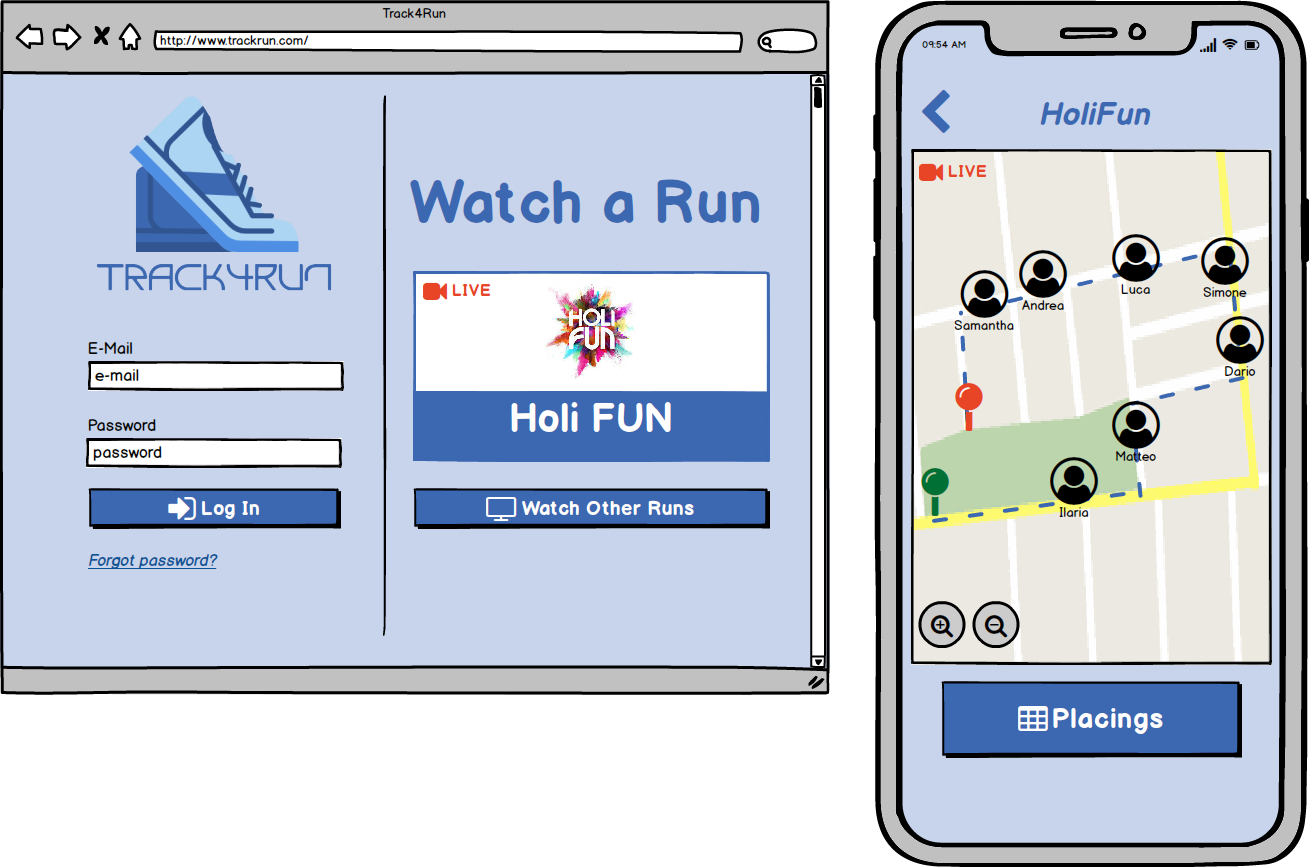
\includegraphics[width=\textwidth]{img/mockup/VisitRun.png}
  \hspace{0.05\linewidth}
  \centering
  \caption{\textit{Run Watching} mockup}
  \label{img:runWatchingMockup}
\end{center}
\end{figure}

\begin{figure}
\begin{center}
  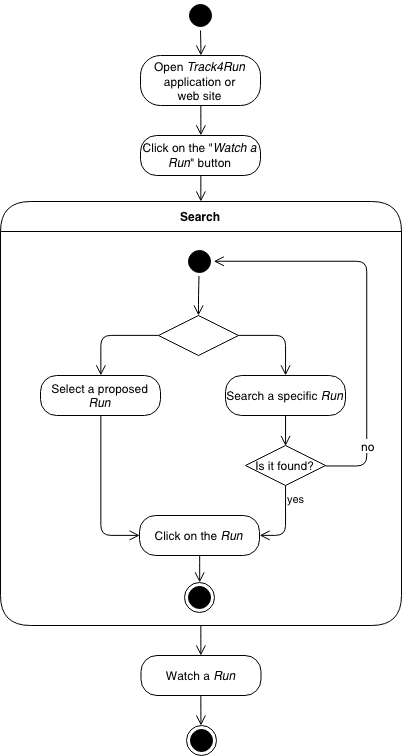
\includegraphics[height=0.6\paperheight]{img/activity/Watching.png}
  \hspace{0.05\linewidth}
  \centering
  \caption{\textit{Run Watching} activity diagram}
  \label{img:runWatchingActivityDiagram}
\end{center}
\end{figure}
